\subsection{Temporal Pooler}


\begin{frame}[c]{Temporal Pooler - Pipeline}
    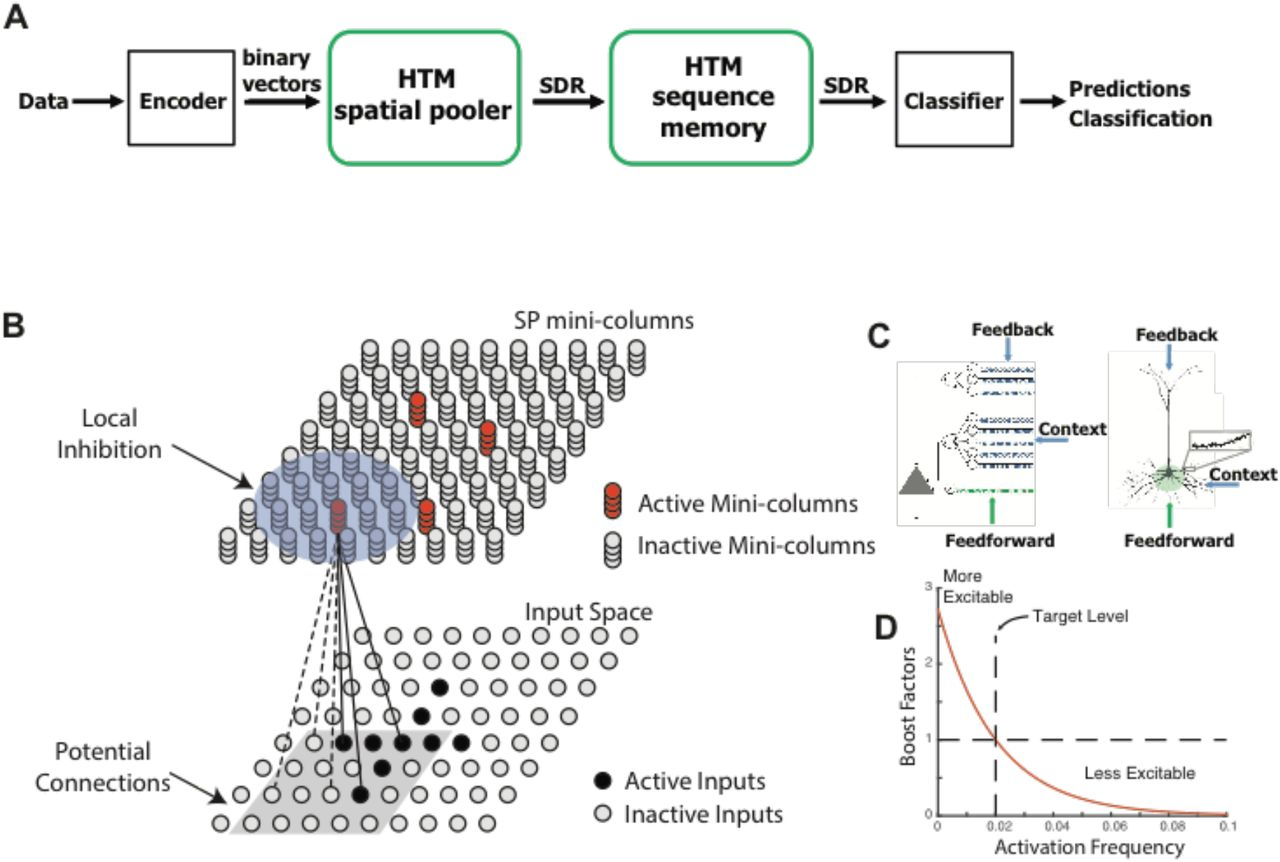
\includegraphics[width=\textwidth, trim = 0 160 0 0,clip]{spatial_pooler} \\
    \normalsize
    Image adapted from \cite{cui2017htm}.
\end{frame}


\begin{frame}[c]{Temporal Pooler - Introduction}
    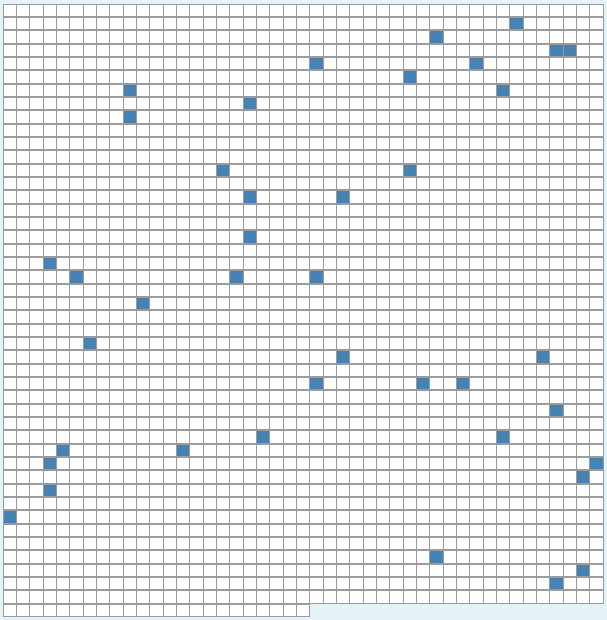
\includegraphics[height=0.9\textheight]{sdr_example}
\end{frame}


\begin{frame}[c]{Temporal Pooler - Introduction}
    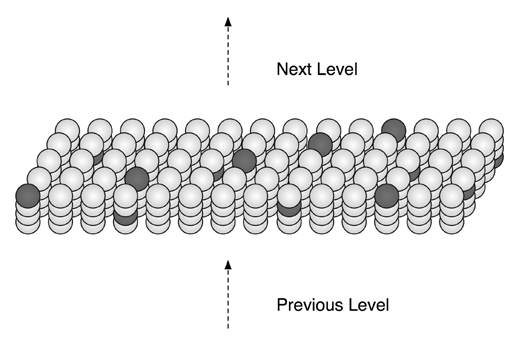
\includegraphics[width=0.95\textwidth]{region_sparse}
\end{frame}


\begin{frame}[c]{Temporal Pooler - Steps}
    \Large
    \begin{enumerate}[<+(1)->]
        \item Form representation in context of previous states
        \item Form predictions based on previous inputs
    \end{enumerate}
\end{frame}


\begin{frame}[c]{Temporal Pooler - Selecting Winner Cells}
    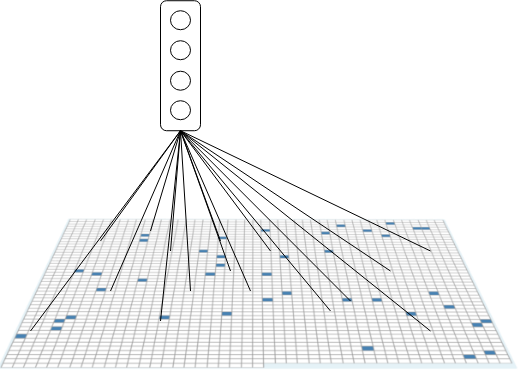
\includegraphics[height=0.9\textheight]{one_left}
\end{frame}

\begin{frame}[c]{Temporal Pooler - Selecting Winner Cells}
    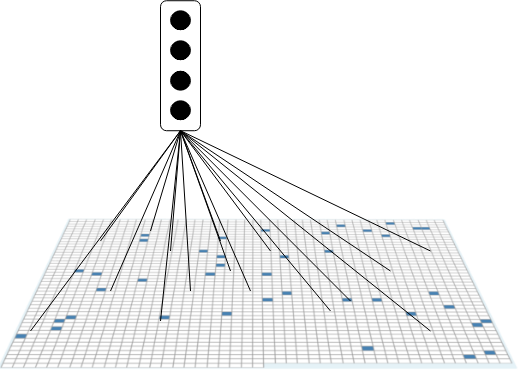
\includegraphics[height=0.9\textheight]{one_left_burst}
\end{frame}

\begin{frame}[c]{Temporal Pooler - Selecting Winner Cells}
    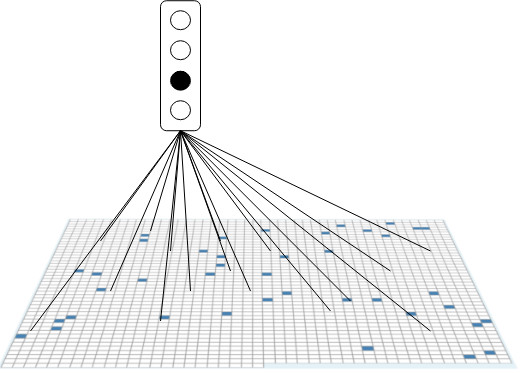
\includegraphics[height=0.9\textheight]{one_left_winner}
\end{frame}

\begin{frame}[c]{Temporal Pooler - Selecting Winner Cells}
    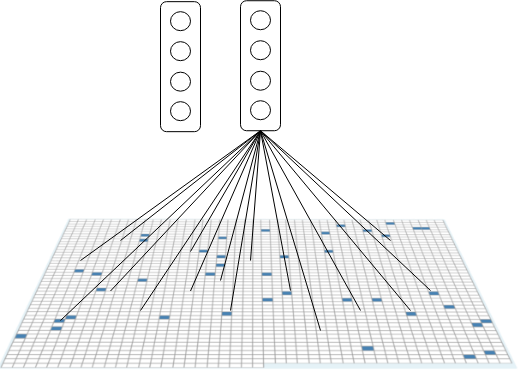
\includegraphics[height=0.9\textheight]{two_left_middle}
\end{frame}

\begin{frame}[c]{Temporal Pooler - Selecting Winner Cells}
    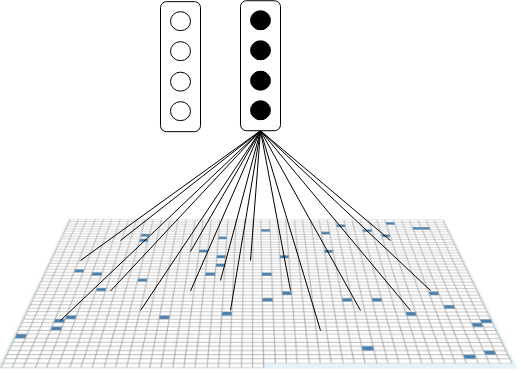
\includegraphics[height=0.9\textheight]{two_left_middle_burst}
\end{frame}

\begin{frame}[c]{Temporal Pooler - Selecting Winner Cells}
    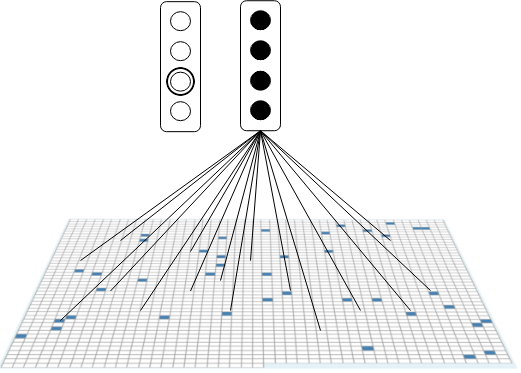
\includegraphics[height=0.9\textheight]{two_left_last_middle_burst}
\end{frame}

\begin{frame}[c]{Temporal Pooler - Selecting Winner Cells}
    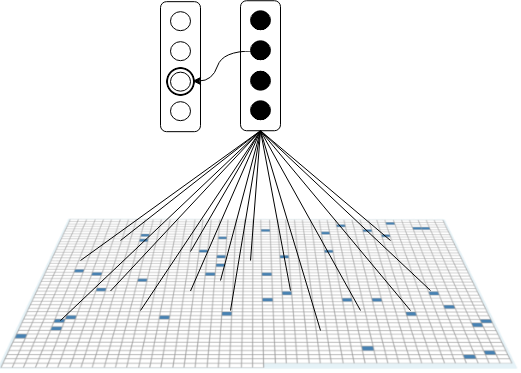
\includegraphics[height=0.9\textheight]{two_left_last_middle_burst_arrow}
\end{frame}

\begin{frame}[c]{Temporal Pooler - Selecting Winner Cells}
    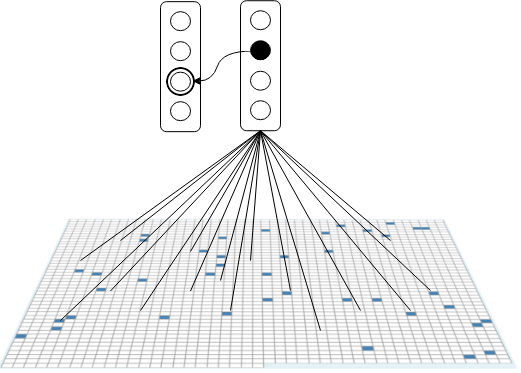
\includegraphics[height=0.9\textheight]{two_left_last_middle_one_arrow}
\end{frame}

\begin{frame}[c]{Temporal Pooler - Selecting Winner Cells}
    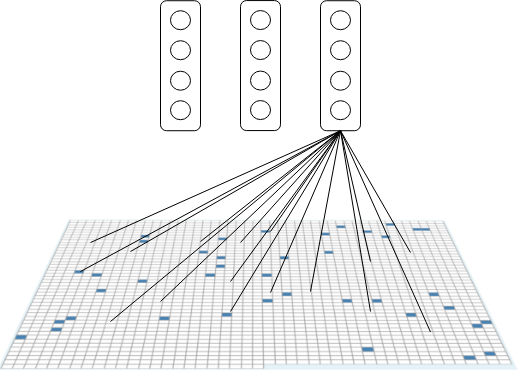
\includegraphics[height=0.9\textheight]{three}
\end{frame}

\begin{frame}[c]{Temporal Pooler - Selecting Winner Cells}
    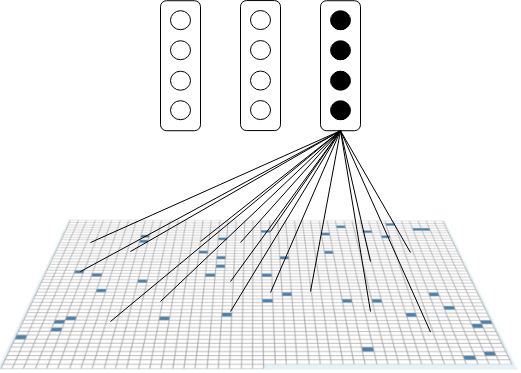
\includegraphics[height=0.9\textheight]{three_burst}
\end{frame}

\begin{frame}[c]{Temporal Pooler - Selecting Winner Cells}
    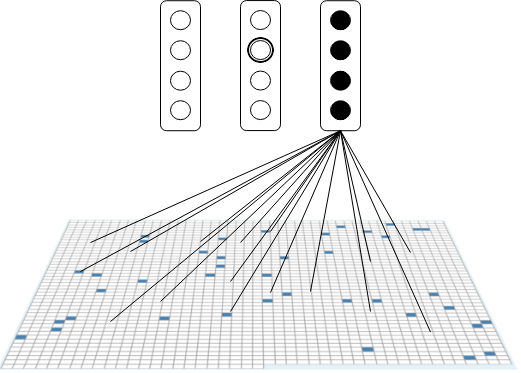
\includegraphics[height=0.9\textheight]{three_last_burst}
\end{frame}

\begin{frame}[c]{Temporal Pooler - Selecting Winner Cells}
    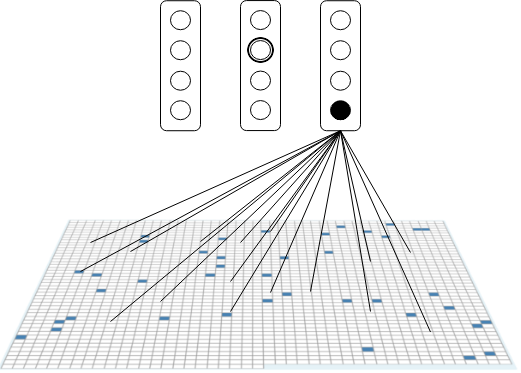
\includegraphics[height=0.9\textheight]{three_last_active}
\end{frame}

\begin{frame}[c]{Temporal Pooler - Selecting Winner Cells}
    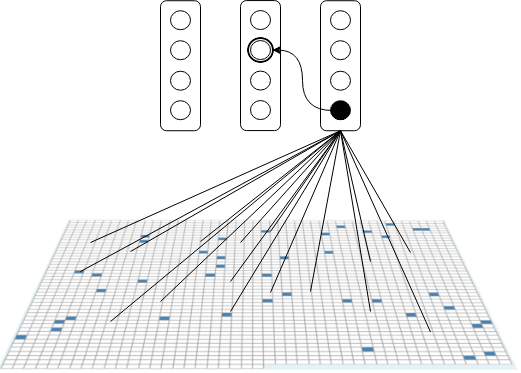
\includegraphics[height=0.9\textheight]{three_last_active_arrow}
\end{frame}

\begin{frame}[c]{Temporal Pooler - Selecting Winner Cells}
    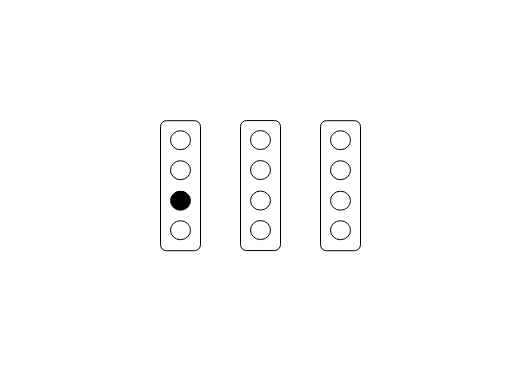
\includegraphics[height=0.9\textheight]{three_without_active}
\end{frame}

\begin{frame}[c]{Temporal Pooler - Selecting Winner Cells}
    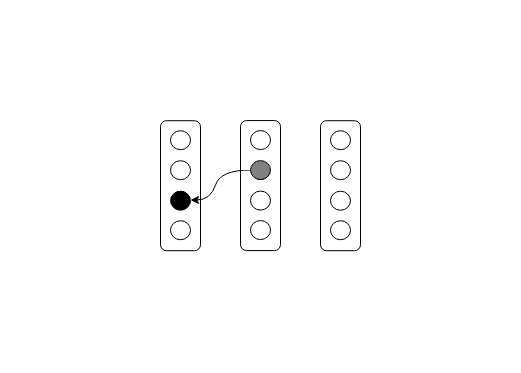
\includegraphics[height=0.9\textheight]{three_predicting}
\end{frame}

\begin{frame}[c]{Temporal Pooler - Selecting Winner Cells}
    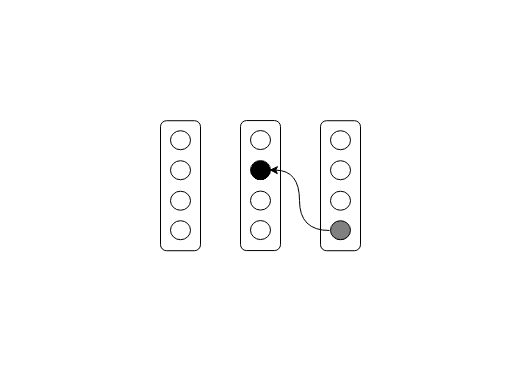
\includegraphics[height=0.9\textheight]{three_predicting_2}
\end{frame}




% \begin{frame}[c]{Temporal Memory - Examples}
%     \Large
%     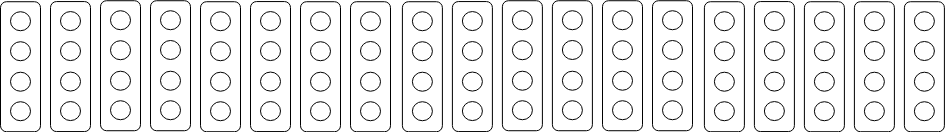
\includegraphics[width=\textwidth]{multiple_cols}
%     \vfill
% \end{frame}


\begin{frame}[c]{Temporal Memory - Example I}
    \Large

    \begin{tabular}{llll}
        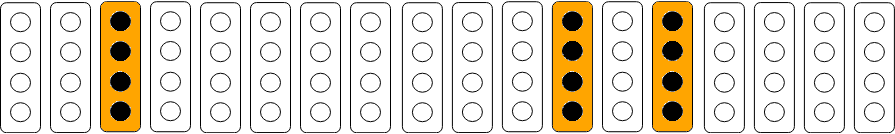
\includegraphics[width=0.23\textwidth]{active_we} &
        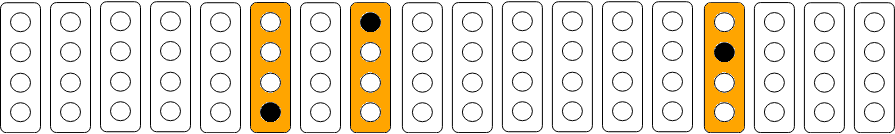
\includegraphics[width=0.23\textwidth]{active_are_2} &
        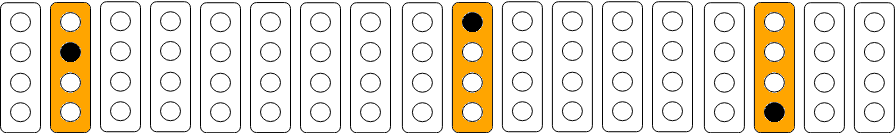
\includegraphics[width=0.23\textwidth]{active_very_2} &
        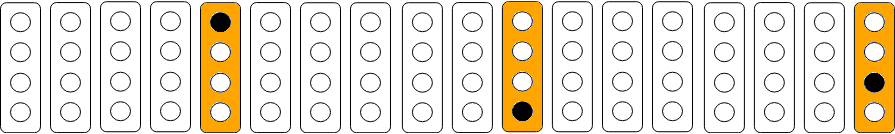
\includegraphics[width=0.23\textwidth]{active_busy} \\
        We & are & very & busy
    \end{tabular}

    \pause
    \vfill

    \begin{tabular}{llll}
        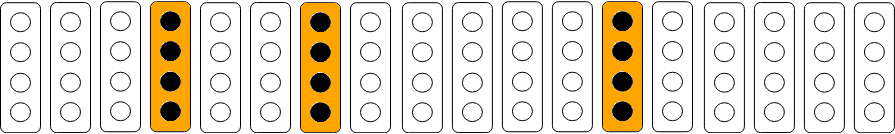
\includegraphics[width=0.23\textwidth]{active_you} &
        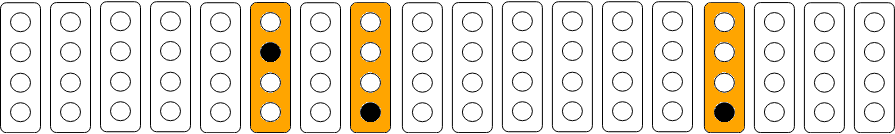
\includegraphics[width=0.23\textwidth]{active_are_1} &
        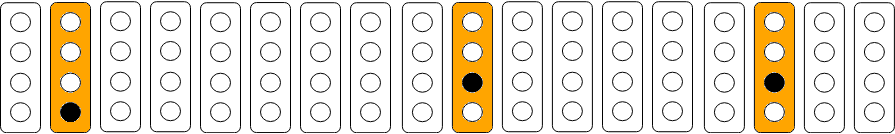
\includegraphics[width=0.23\textwidth]{active_very_1} &
        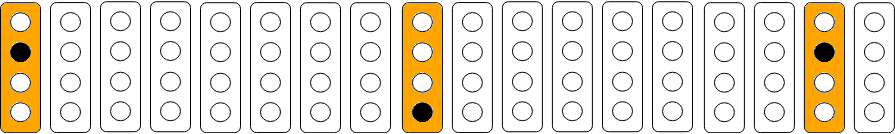
\includegraphics[width=0.23\textwidth]{active_knowledgeable} \\
        You & are & very & knowledgeable
    \end{tabular}
\end{frame}


\begin{frame}[c]{Temporal Memory - Example I}
    \Large
    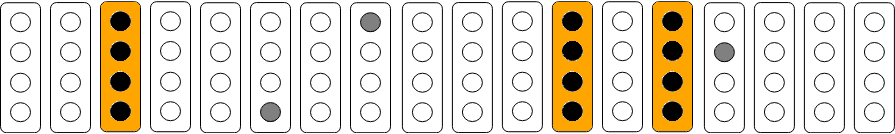
\includegraphics[width=\textwidth]{active_we_predicted_are2} \\
    We
\end{frame}


\begin{frame}[c]{Temporal Memory - Example I}
    \Large
    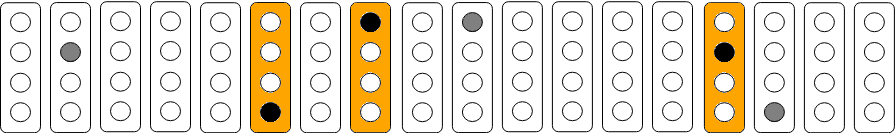
\includegraphics[width=\textwidth]{active_are2_predicted_very2} \\
    We are
\end{frame}


\begin{frame}[c]{Temporal Memory - Example I}
    \Large
    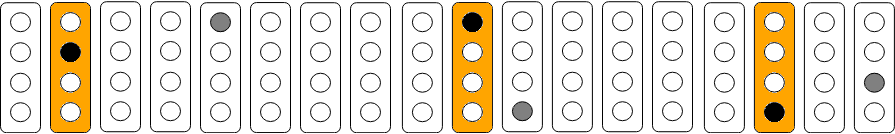
\includegraphics[width=\textwidth]{active_very2_predicted_busy} \\
    We are very
\end{frame}


\begin{frame}[c]{Temporal Memory - Example I}
    \Large
    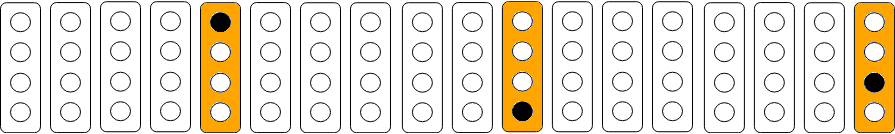
\includegraphics[width=\textwidth]{active_busy} \\
    We are very busy
\end{frame}


\begin{frame}[c]{Temporal Memory - Example I}
    \Large

    \begin{tabular}{llll}
        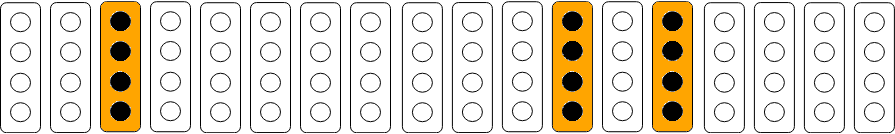
\includegraphics[width=0.23\textwidth]{active_we} &
        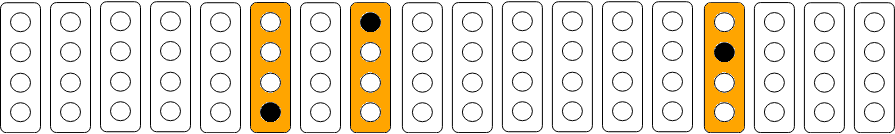
\includegraphics[width=0.23\textwidth]{active_are_2} &
        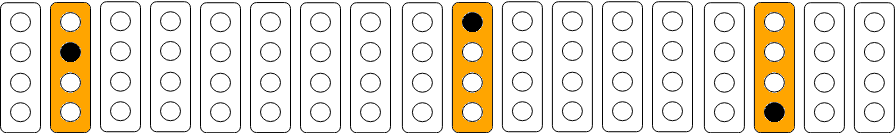
\includegraphics[width=0.23\textwidth]{active_very_2} &
        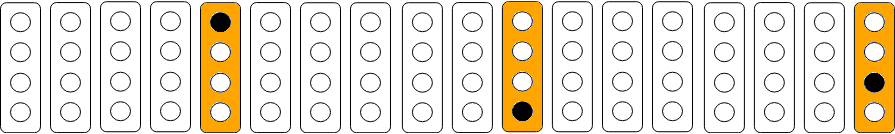
\includegraphics[width=0.23\textwidth]{active_busy} \\
        We & are & very & busy
    \end{tabular}

    \begin{tabular}{llll}
        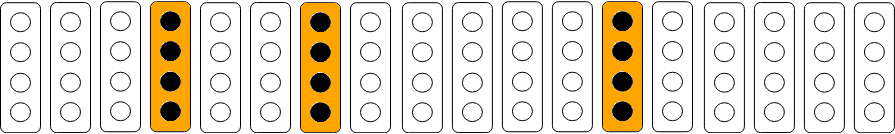
\includegraphics[width=0.23\textwidth]{active_you} &
        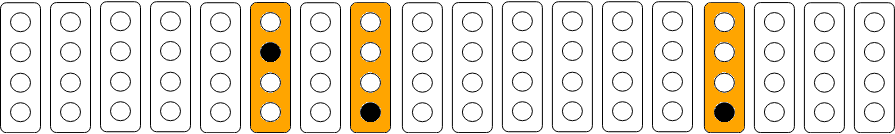
\includegraphics[width=0.23\textwidth]{active_are_1} &
        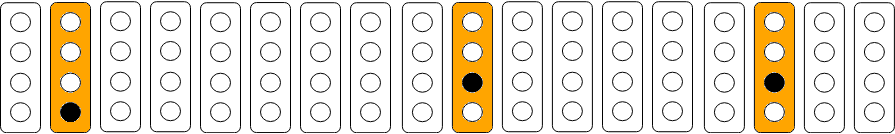
\includegraphics[width=0.23\textwidth]{active_very_1} &
        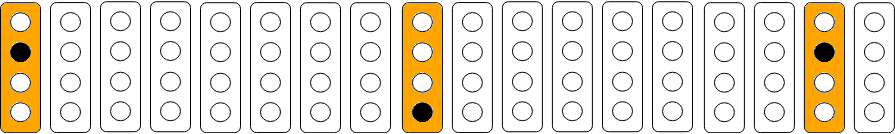
\includegraphics[width=0.23\textwidth]{active_knowledgeable} \\
        You & are & very & knowledgeable
    \end{tabular}
    \vfill
    \phantom{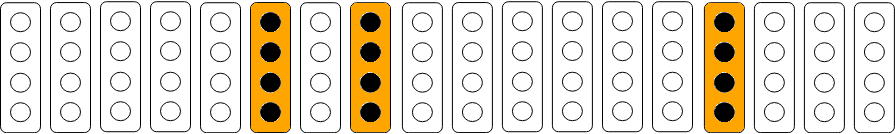
\includegraphics[width=\textwidth]{active_are_bursting} \\ are}
\end{frame}


\begin{frame}[c]{Temporal Memory - Example I}
    \Large

    \begin{tabular}{llll}
        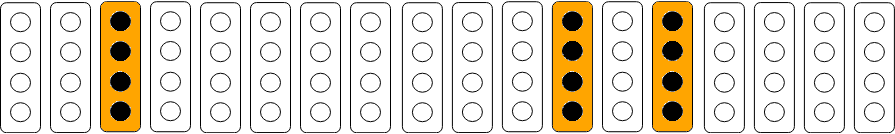
\includegraphics[width=0.23\textwidth]{active_we} &
        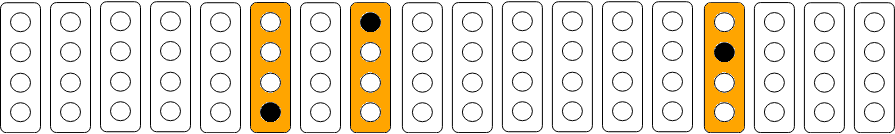
\includegraphics[width=0.23\textwidth]{active_are_2} &
        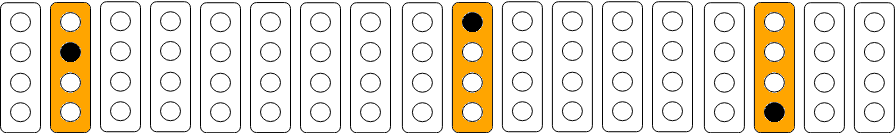
\includegraphics[width=0.23\textwidth]{active_very_2} &
        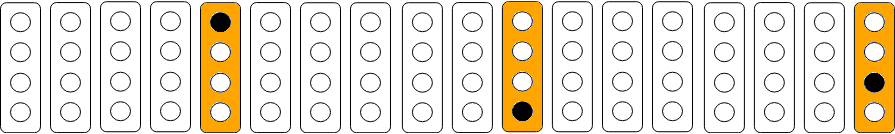
\includegraphics[width=0.23\textwidth]{active_busy} \\
        We & are & very & busy
    \end{tabular}

    \begin{tabular}{llll}
        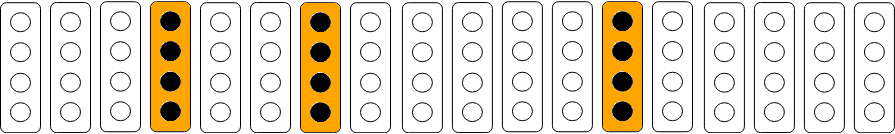
\includegraphics[width=0.23\textwidth]{active_you} &
        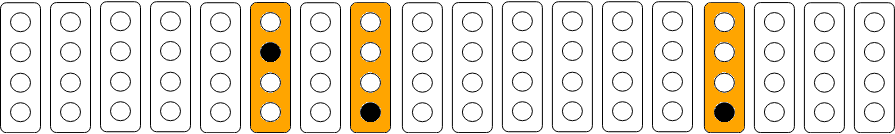
\includegraphics[width=0.23\textwidth]{active_are_1} &
        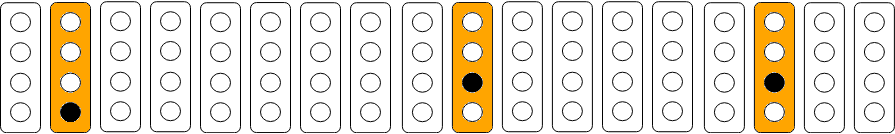
\includegraphics[width=0.23\textwidth]{active_very_1} &
        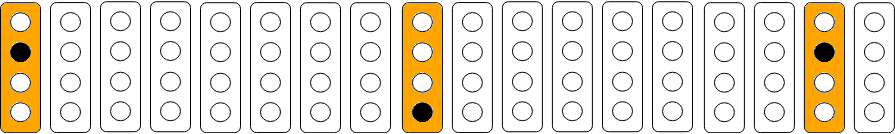
\includegraphics[width=0.23\textwidth]{active_knowledgeable} \\
        You & are & very & knowledgeable
    \end{tabular}
    \vfill
    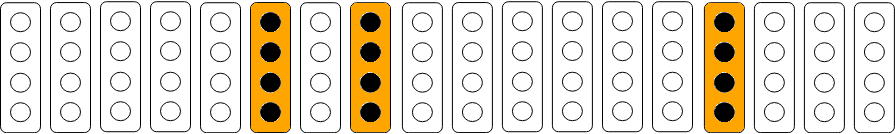
\includegraphics[width=\textwidth]{active_are_bursting} \\ are
\end{frame}


\begin{frame}[c]{Temporal Memory - Example I}
    \Large

    \begin{tabular}{llll}
        \includegraphics[width=0.23\textwidth]{active_we} &
        \includegraphics[width=0.23\textwidth]{active_are_2} &
        \includegraphics[width=0.23\textwidth]{active_very_2} &
        \includegraphics[width=0.23\textwidth]{active_busy} \\
        We & are & very & busy
    \end{tabular}

    \begin{tabular}{llll}
        \includegraphics[width=0.23\textwidth]{active_you} &
        \includegraphics[width=0.23\textwidth]{active_are_1} &
        \includegraphics[width=0.23\textwidth]{active_very_1} &
        \includegraphics[width=0.23\textwidth]{active_knowledgeable} \\
        You & are & very & knowledgeable
    \end{tabular}
    \vfill
    \includegraphics[width=\textwidth]{active_are_bursting_predict} \\
    are
\end{frame}


\begin{frame}[c]{Temporal Memory - Example I}
    \Large

    \begin{tabular}{llll}
        \includegraphics[width=0.23\textwidth]{active_we} &
        \includegraphics[width=0.23\textwidth]{active_are_2} &
        \includegraphics[width=0.23\textwidth]{active_very_2} &
        \includegraphics[width=0.23\textwidth]{active_busy} \\
        We & are & very & busy
    \end{tabular}

    \begin{tabular}{llll}
        \includegraphics[width=0.23\textwidth]{active_you} &
        \includegraphics[width=0.23\textwidth]{active_are_1} &
        \includegraphics[width=0.23\textwidth]{active_very_1} &
        \includegraphics[width=0.23\textwidth]{active_knowledgeable} \\
        You & are & very & knowledgeable
    \end{tabular}
    \vfill
    \includegraphics[width=\textwidth]{active_very_predict_two} \\ very
\end{frame}


\begin{frame}[c]{Temporal Memory - Advanced}
    \Large
    \begin{itemize}[<+(1)->]
        \item Within a region
        \item But also across
        \item Up and Down
        \item There are much more connections DOWN than UP
        \item In fact, about 90\% go either sideways or DOWN
    \end{itemize}
\end{frame}


\begin{frame}[c]{Temporal Memory - Example II}
    \Large
    \begin{itemize}[<+(1)->]
        \item I \textbf{ate} a pear
        \item I have \textbf{eight} pears
    \end{itemize}
    \vfill
    \begin{itemize}[<+(1)->]
        \item I ...
        \item I have ...
    \end{itemize}
    \pause
    Temporal predictions add to the threshold for the spatial pooler!
    % example for predicting different concepts, included in spatial pooler counting as well
\end{frame}


\begin{frame}[c]{Temporal Memory - SDRs Advanced II}
    \Large
    \textbf{Q:} If you have an SDR with 10 000 Cells and 200 active, how much difference would saving only 20 of them make?
    \newline
    \pause
    \newline
    \textbf{A:} Due to the property of SDRs, it is {\em very} unlikely that they activate in a totally unrelated pattern.
\end{frame}





%         \item If there are no exact matches (would have been predicted and direct winner otherwise), take near matches
%         \item No matching segments at all: select cell with fewest segments (randomly select in case of tie)
%                 Create or grow synapses/segments to winning cells from last step









\begin{frame}[c]{Temporal Pooler - Closing notes}
    \begin{itemize}[<+(1)->]
        \item Every Column will have a winner cell
        \item Bursting can happen on single columns as well
    \end{itemize}
\end{frame}


